\newcommand{\econtexRoot}{.}
% The \commands below are required to allow sharing of the same base code via Github between TeXLive on a local machine and ShareLaTeX.  This is an ugly solution to the requirement that custom LaTeX packages be accessible, and that ShareLaTeX seems to ignore symbolic links (even if they are relative links to valid locations)
\providecommand{\econtex}{\econtexRoot/texmf-local/tex/latex/econtex}
\providecommand{\econtexSetup}{\econtexRoot/texmf-local/tex/latex/econtexSetup}
\providecommand{\econtexShortcuts}{\econtexRoot/texmf-local/tex/latex/econtexShortcuts}
\providecommand{\econtexBibMake}{\econtexRoot/texmf-local/tex/latex/econtexBibMake}
\providecommand{\econtexBibStyle}{\econtexRoot/texmf-local/bibtex/bst/econtex}
\providecommand{\notes}{\econtexRoot/texmf-local/tex/latex/handout}
\providecommand{\handoutSetup}{\econtexRoot/texmf-local/tex/latex/handoutSetup}
\providecommand{\handoutShortcuts}{\econtexRoot/texmf-local/tex/latex/handoutShortcuts}
\providecommand{\handoutBibMake}{\econtexRoot/texmf-local/tex/latex/handoutBibMake}
\providecommand{\handoutBibStyle}{\econtexRoot/texmf-local/bibtex/bst/handout}

  
\documentclass[titlepage]{\econtex}\newcommand{\texname}{BPP_TimeAgg}
\usepackage{\econtexSetup}\usepackage{\econtexShortcuts}
\usepackage[nolists,nomarkers,tablesonly]{endfloat}
\usepackage{tikz}
\usepackage{caption}
\usepackage{titlesec}
\setcounter{secnumdepth}{4}

\provideboolean{ifWeb}
\setboolean{ifWeb}{false}
\opt{Web}{\setboolean{ifWeb}{true}}

\ifthenelse{\boolean{ifWeb}}{\usepackage{grfext}
\PrependGraphicsExtensions*{.svg,.jpg,.JPG,.png,.PNG,.pdf,.PDF}
}{}


\titleformat{\paragraph}
{\sffamily\mdseries\normalsize}{\theparagraph}{1em}{}
\titlespacing*{\paragraph}
{0pt}{3.25ex plus 1ex minus .2ex}{1.5ex plus .2ex}

\hypersetup{pdfauthor={Edmund Crawley <ecrawle2@jhu.edu>},
            pdftitle={Time Aggregation in Panel Data on Income and Consumption},
            pdfsubject={Time Aggregation in Panel Data on Income and Consumption},
            pdfkeywords={Income, Consumption, Saving; JEL: D12, D31, D91, E21},
            pdfproducer = {LaTeX with hyperref and thumbpdf},
            pdfcreator = {pdflatex}
            }

\newlength\TableWidth

\provideboolean{StandAlone}
\setboolean{StandAlone}{false}
\write18{\TabsDir/StandAloneOff.command} % Tell input files that they are being pulled in from the master (and are not standalone documents)

%rm%\provideboolean{PrintVersion}
%rm%\setboolean{PrintVersion}{false}
%rm%\setboolean{PrintVersion}{true}


\begin{document}\bibliographystyle{\econtexBibStyle}

\input Switches.tex

\begin{verbatimwrite}{\jobname.title}
Time Aggregation in Panel Data on Income and Consumption
\end{verbatimwrite}

\hfill{\tiny \jobname}

\title{Time Aggregation in Panel Data \\ on Income and Consumption}

\ifthenelse{\boolean{ifWeb}}{
\author{
  Edmund Crawley\authNum 
}
}{
\author{
  Edmund Crawley\authNum   \\ {\small JHU and Danmarks Nationalbank}
}
} % End ifWeb

\keywords{Income, Consumption, Saving}
\jelclass{D12, D31, D91, E21}
% \aspublished{Final version as published in [].}

%\date{March 14, 2018}
\maketitle

\begin{abstract}
  \opt{JournalFormatting}{\doublespacing}
%  \begin{verbatimwrite}{./.abstract.metadata} 
    The time aggregation problem. of \cite{working_note_1960}
%  \end{verbatimwrite}{./.abstract.metadata} 
%  \input{./.abstract.metadata}
\end{abstract}


\begin{authorsinfo}
\name{Crawley: Department of Economics, Johns Hopkins University, \href{mailto:ecrawle2@jhu.edu}{\texttt{ecrawle2@jhu.edu}}}
\end{authorsinfo}
\thanks{Thanks to Danmarks Nationalbank for providing financial support}

\titlepagefinish
\setcounter{page}{1}

\pagebreak
%rm%\provideboolean{SlidesInText}
%rm%\setboolean{SlidesInText}{true}
\section{Introduction}
In a short note in Econometrica, \cite{working_note_1960} made the simple but important point that time aggregation can induce serial correlation that is not present in the original series. This fact was readily absorbed by the macroeconomic literature, where such time aggregated series are common (for an example see \cite{campbell_consumption_1989}). Recently, by studying the covariance structure of panel data, much progress has been made in understanding household income and consumption dynamics. However, this literature has not accounted for the serial correlation induced by the time aggregated nature of observed income and consumption data. This oversight can result in significant bias. This paper will focus on the implications of time aggregation for the methodology in \cite{blundell_consumption_2008} (henceforth BPP), but it applies to a broad swath of the literature. I show that the pass through from transitory income to consumption, originally estimated by BPP to be 5\%, is close to 20\% when the serial correlation in the data induced by time aggregation is accounted for.

\subsection{What is Time Aggregation?}
Many observed time series in economics are given at a lower frequency than the underlying data that generates them. For example, income is often observed at an annual frequency when it may in fact consist of paychecks arriving at a monthly, biweekly or irregular timetable. The transform income into an annual frequency we sum up all the income that was received by a household during the year, a process known as time aggregation. The key insight of \cite{working_note_1960} is that even if there is no correlation between changes in income at the underlying frequency, the time resulting time aggregated series will show positive autocorrelation. The intuition behind this can be seen in figure \ref{fig:TimeAggExample} showing an income process that begins at zero and increases to one in the second year. The top left graph shows the path of income if the shock occurs exactly at the start of the second year, and the bottom left graph shows the time aggregated process exactly mirrors that. There is no income in the first year and one unit of income in each of the second and third years. The top right shows an alternative income process in which the shock occurs half way through the second year. Now the resulting time aggregated process (bottom right) does not mirror the underlying. As before there is no income in the first year, but in the second year the individual receives an income of one for half the year, resulting in a time aggregated income of 0.5. In the third year the individual receives an income of one for the entire year, and hence a time aggregated income of one. If we can only see the time aggregated process, when we observe income increasing from year one to year two we do not know if the shock occurred at the beginning of the year or half way through. If it occurred at the beginning of the year, as in the left hand graphs of figure \ref{fig:TimeAggExample}, then we would not expect to see any further increase in the time aggregated process associated with it. However, if it occurred half way through, as in the right hand graphs of figure \ref{fig:TimeAggExample}, we would only have observed half the total increase in income and would expect the time aggregated process to continue to increasing in the following period. Therefore, assuming there is some positive probability that the shock occurred half way through the second period, we would expect to see further increases in the observed process. This is how time aggregation induces serial correlation in the first difference of an observed process even when the underlying process is a random walk. Section \ref{TimeAggRandomWalk} lays this out formally and shows that this autocorrelation tends to $\frac{1}{4}$ as the number of time subdivisions increases to infinity.
\begin{figure}
	\caption{Time Aggregation Induces Serial Correlation}
	\label{fig:TimeAggExample}
	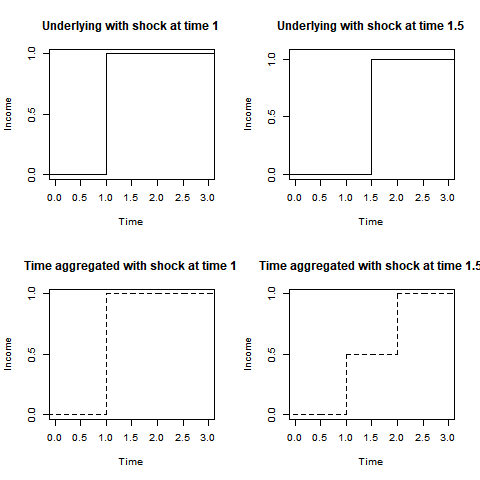
\includegraphics[width=1\textwidth]{../Code/Figures/TimeAggExample.png}
\end{figure}

\subsection{Relation to the Literature}

\section{Time Aggregated Random Walk} \label{TimeAggRandomWalk}
I this section I formally prove that a time aggregated random walk is autocorrelated and show that this autocorrelation tends to $\frac{1}{4}$ as the number of time subdivisions increases to infinity. I will also introduce continuous time notation that will be used for the underlying model in section \ref{BPP}.

\subsection{The two sub-division case}
I begin with the two-subdivision case. The underlying income process follows a random walk at discrete time periods $t\in \{0,1,2,3,...\}$:
\begin{align*}
y_t = \begin{cases}
0 \qquad & \text{if } t=0\\
	y_{t-1} + \varepsilon_t & \text{otherwise}
	\end{cases}
\end{align*}
where $\varepsilon_t$ is i.i.d. and has variance $\sigma^2$. The  time aggregated process is observed every two periods at $T\in\{2,4,6,...\}$ and is equal to the sum of income over the two periods leading up to it:
\begin{align*}
y_T^{obs} = y_T + y_{T-1}
\end{align*}
The observed income change is given by:
\begin{align*}
\Delta^2 y_T^{obs} &= y_T^{obs} - y_{T-2}^{obs} \\
&= \varepsilon_T + 2\varepsilon_{T-1} + \varepsilon_{T-2}
\end{align*}
This allows for easy calculation of the serial correlation:
\begin{align*}
\mathrm{Cov}(\Delta^2 y_T^{obs},\Delta^2 y_{T-2}^{obs}) &= \sigma^2 \\
\mathrm{Var}(\Delta^2 y_T^{obs}) &= \sigma^2 + 4\sigma^2 + \sigma^2 \\
&= 6\sigma^2 \\
\mathrm{Corr}(\Delta^2 y_T^{obs},\Delta^2 y_{T-2}^{obs}) &= \frac{1}{6}
\end{align*}

\subsection{The N sub-division case}
The two sub-division case easily extends to N sub-divisions. Using the same underlying income process, the observable income process is now aggregated over N periods:
\begin{align*}
y_T^{obs} = \sum_{t=T-N+1}^{T} y_t
\end{align*}
So that the observed change in income is:
\begin{align*}
\Delta^N y_T^{obs} &= \sum_{t=T-N+1}^{T} y_t - y_{t-N} \\
&= \varepsilon_T + \varepsilon_{T-1} +  \qquad...  \qquad+ \varepsilon_{T-N+2} + \varepsilon_{T-N+1} \\
& \qquad \   +  \varepsilon_{T-1} + \varepsilon_{T-2}  + \qquad...  \qquad \quad \ + \varepsilon_{T-N+1} + \varepsilon_{T-N} \\
& \qquad \qquad  \quad \ \, +  \varepsilon_{T-2} + \varepsilon_{T-3} + \qquad ... \\
& \qquad \qquad \qquad \qquad \qquad \qquad ...\\
& \qquad \qquad \qquad \qquad \qquad \qquad \qquad \qquad \ +  \varepsilon_{T-N+1} +\qquad ...  \qquad + \varepsilon_{T-2N+2} \\
&= N \varepsilon_{T-N+1} + \sum_{i=1}^{N-1} i\Big(\varepsilon_{T-i+1} + \varepsilon_{T-2N+i+1} \Big)
\end{align*}
We can now calculate the autocorrelation:
\begin{align*}
\mathrm{Cov}(\Delta^N y_T^{obs},\Delta^N y_{T-N}^{obs}) &=\sum_{i=1}^{N-1} i(N-i) \sigma^2 \\
&=  \frac{N(N^2-1)}{6} \sigma^2 \\
\mathrm{Var}(\Delta^N y_T^{obs}) &= N^2\sigma^2 + 2\sum_{i=1}^{N-1} i^2 \sigma^2 \\
&= \frac{N(2N^2+1)}{3}\sigma^2 \\
\mathrm{Corr}(\Delta^N y_T^{obs},\Delta^N y_{T-N}^{obs}) &= \frac{N^2-1}{2(2N^2+1)} \rightarrow \frac{1}{4} \text{ as } N \rightarrow \infty
\end{align*}
\subsection{The Continuous Time Case}
It will turn out to be significantly simpler to work with a model in which shocks can occur at any point in continuous time. Here I introduce some notation for such a model, and show that it gives a good approximation even if the actual underlying process is discrete (say quarterly or monthly).

The underlying income process will be modeled as a martingale process in continuous time, $y_t$, where for all  $s_1>s_2>s_3>s_4>0$:
\begin{align*}
\mathrm{Var}(y_{s_1}-y_{s_2})=(s_1-s_2)\sigma^2 \\
\mathrm{Cov}(y_{s_1}-y_{s_2},y_{s_3}-y_{s_4}) = 0 \\
y_s = 0 \qquad \text{if } s<0
\end{align*}
The process has independent increment increments. A Brownian motion would satisfy these criteria, but although in continuous time there is no restriction that it is a continuous process (it may have jumps).\footnote{Note that such a process will take both positive and negative values, and therefore may not be a good choice for an income process. In appendix ******* I show that under certain assumptions the same results approximately hold when shocks are multiplicative rather than additive.} The observed income process is the sum of income over a year:
\begin{align*}
\bar{y}_T &= \int_{T-1}^{T} y_t dt \\
&= \int_{T-1}^{T} \int_{0}^{t} dy_s dt 
\end{align*}
So that:
\begin{align*}
\Delta \bar{y}_T &= \int_{T-1}^{T} \int_{0}^{t} dy_s dt - \int_{T-2}^{T-1} \int_{0}^{t} dy_s dt \\
&= \int_{T-1}^{T} \int_{t-1}^{t} dy_s dt \\
&= \int_{T-1}^{T} (T-s) dy_s + \int_{T-2}^{T-1} (s-(T-2)) dy_s 
\end{align*}
The autocorrelation can now be calculated:
\begin{align*}
\mathrm{Cov}(\Delta \bar{y}_T,\Delta \bar{y}_{T-1}) &=  \int_{T-2}^{T-1} (T-1-s)(s-(T-2)) \sigma^2 dt \\
&= \frac{1}{6}\sigma^2 \\
\mathrm{Var}(\Delta \bar{y}_T) &= \int_{T-1}^{T} (T-s)^2 \sigma^2 dt + \int_{T-2}^{T-1} (s-(T-2))^2 \sigma^2 dt \\
&= \frac{2}{3}\sigma^2 \\
\mathrm{Corr}(\Delta \bar{y}_T,\Delta \bar{y}_{T-1}) &= \frac{1}{4}
\end{align*}
Which is unsurprisingly the same as the limit of the autocorrelation in the N sub-periods case.
\begin{figure}
	\caption{Induced Autocorrelation for different N}
	\label{fig:InducedAutocorrelation}
	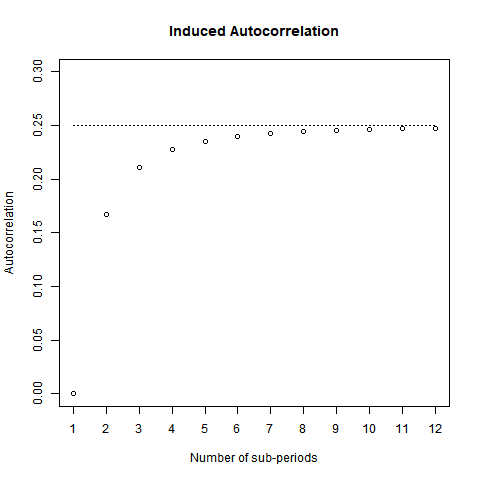
\includegraphics[width=1\textwidth]{../Code/Figures/InducedAutocorrelation.png}
\end{figure}
Figure \ref{fig:InducedAutocorrelation} shows how fast the N sub-period case converges towards the continuous time case. When $N=1$ the time aggregated process is the same as the underlying random walk so the autocorrelation is zero. When income is quarterly ($N=4$) the autocorrelation is 0.23 and is closely approximated by the continuous time model. With monthly ($N=12$) or higher frequency for income shocks the discrete and continuous models are almost indistinguishable. 

\section{Time Aggregation in \cite{blundell_consumption_2008}} \label{BPP}


\processdelayedfloats

\small
\bibliography{AllPapers}
\normalsize

\pagebreak
\appendix

\section*{Appendix}


\end{document}









